\documentclass[twocolumn]{article}
\usepackage{fullpage}
\usepackage{graphicx}
\usepackage{framed}
\usepackage{tcolorbox}
\usepackage{verbatim}
\usepackage{fancyvrb}
\usepackage{comment}
\usepackage{amsmath}
\usepackage{geometry}
\usepackage{enumitem}
\usepackage{etoolbox}
% \usepackage{bold-extra}
\usepackage{xcolor}
\usepackage[colorlinks=true, linkcolor=blue, urlcolor=blue, citecolor=violet]{hyperref}

% \renewcommand{\topfraction}{.99}
% \renewcommand{\bottomfraction}{.99}
% \renewcommand{\textfraction}{.01}
% \renewcommand{\floatpagefraction}{.9}
% \renewcommand{\dbltopfraction}{.99}
% \renewcommand{\dblfloatpagefraction}{.9}

\widowpenalty 10000
\clubpenalty 10000
\tolerance=9999
\newcommand{\tm}{\raisebox{.9ex}{\tiny tm}}

\newcommand{\harmonysource}[1]{
\begin{tabbing}
XX\=XXX\=XXX\kill
    \input{sources/#1.tex}
\end{tabbing}
}

\newcommand{\harmonylink}[1]{%
[\href{https://harmony.cs.cornell.edu/#1}{\underline{#1}}]%
}

\newcommand{\harmonyref}[2]{%
\href{https://harmony.cs.cornell.edu/output/#1}{\underline{#2}}%
}

\newenvironment{code}{
\tcolorbox
}{
\endtcolorbox
}

\title{Concurrent Programming in Harmony}
\author{Robbert van Renesse \and William Ma \and Kevin Sun \and Anthony Yang}

\begin{document}
\maketitle

<{:const:tas}>
<{:const:cas}>
<{:const:BinSem}>
<{:const:Semaphore}>
<{:const:__init__}>
<{:const:p}>
<{:const:hello}>

\begin{figure*}
\begin{center}
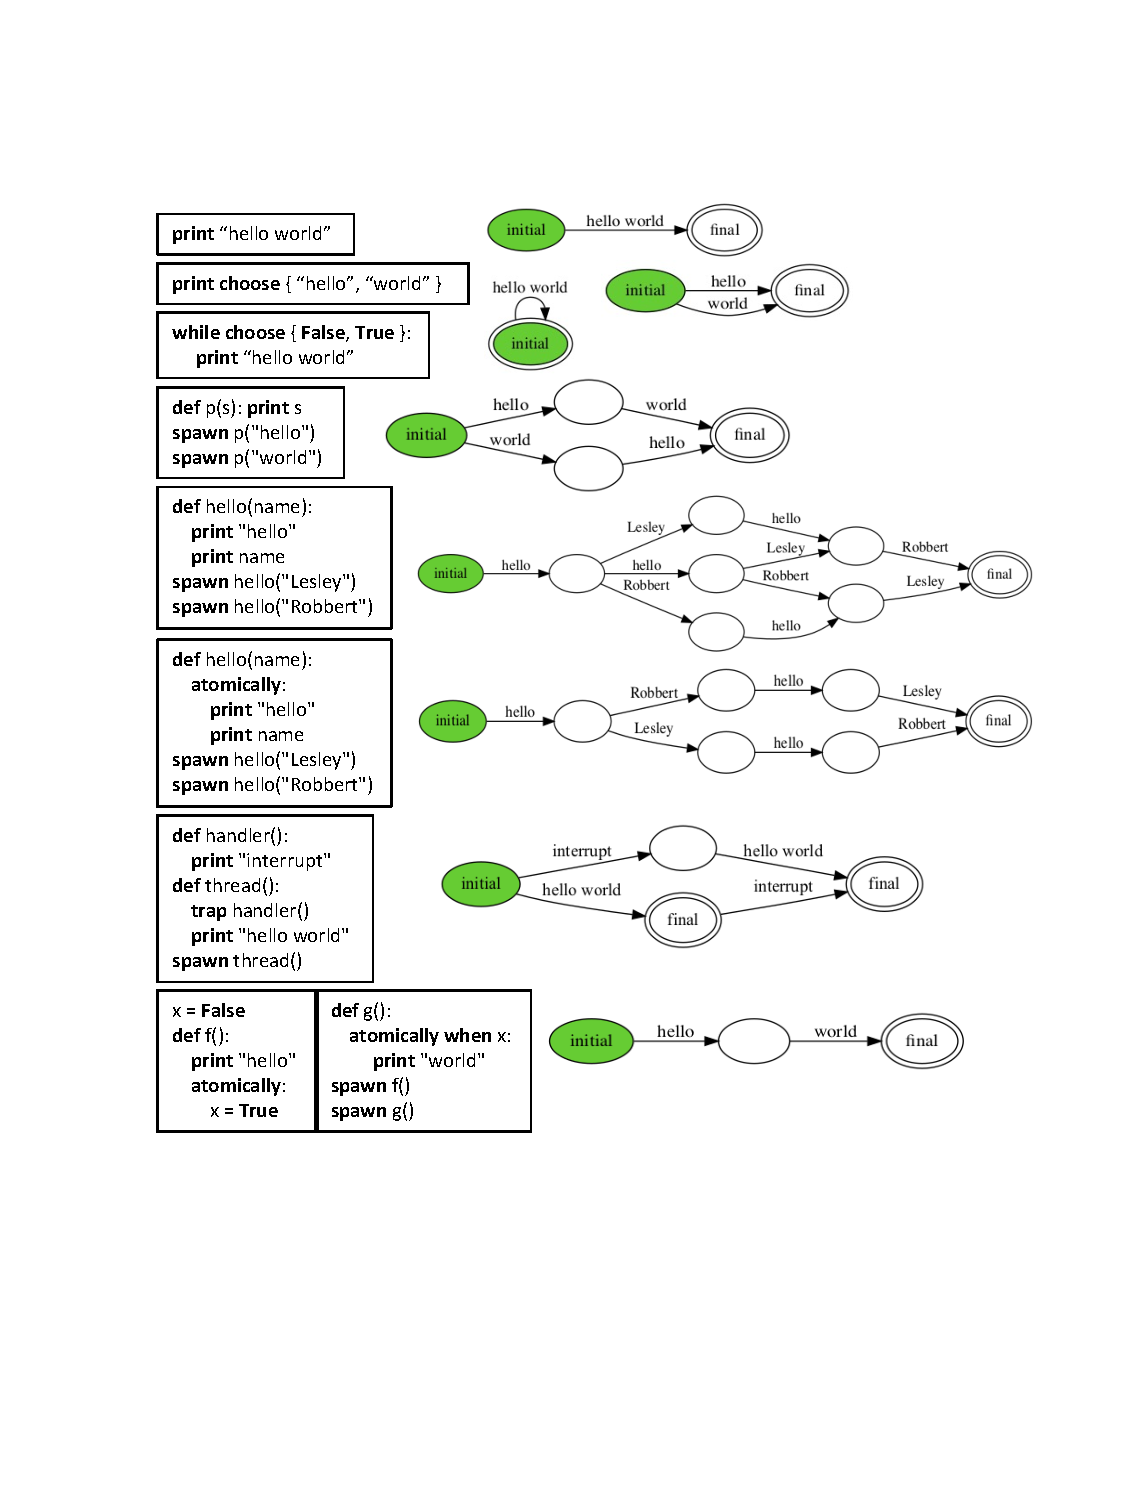
\includegraphics[width=.9\textwidth]{hello.pdf}
\end{center}
\caption{A selection of Harmony programs and their outputs}
\label{fig:helloworld}
\end{figure*}

\section{Introduction}

\emph{Harmony} is a Python-like programming language designed to teach
concurrent and distributed programming to students who do not have a
background in formal methods.  Harmony programs are model checked.
Without any special annotation, Harmony can diagnose a large variety
of problems:
\begin{itemize}
\item ``Silly errors'': accessing non-existent variables,
divide-by-zero, out-of-bounds array access, trying to multiply two lists
with one another, and many more.
\item Safety violations due to assertions failing, such as an assertion to ensure mutual exclusion.
\item Liveness violations (deadlock).
\item Faulty behaviors: implementation has behaviors not seen with specification, such as violations of linearizability;
\item Incomplete behaviors: specification has behaviors not seen with implementation, such as multiple readers not able to get a reader/writer lock simultaneously;
\item Data races: variables accessed without a lock.
\item Busy Waiting: waiting for a condition without blocking.
\end{itemize}

Harmony programs have three sources of non-determinism:
<{choose}> operations that select a value from a set,
\emph{interleaving} due to multi-threading, and \emph{interrupts}.
\autoref{fig:helloworld} demonstrates the <{choose}> and the <{spawn}>
statements.  Since Harmony programs are model-checked and multiple
executions are explored across a finite set of states, the output of a
Harmony program is a finite automaton that describes all possible
outputs of the program.  Groups of statements can be made atomic
using the <{atomically}> keyword.  Finally, Harmony supports a thread
waiting until some condition is reached with the <{when}> statement.

Harmony programs compile to a virtual machine.  The Harmony virtual
machine is formally specified using TLA+, allowing Harmony programs
to run using TLC, the model checker that comes with the TLA+
toolbox.  Harmony has its own custom concurrent model checker that
scales significantly better for Harmony programs.

The Harmony language can be used both to \emph{specify} desired
behaviors and to \emph{implement} them.  To check that the implementation
satisfies the specification, the programmer writes a test program that
systematically checks available operations and prints the results.
The test program is first run against the specification, generating
a \emph{behavior automaton}.  The same test program is then run
against the implementation, along with the behavior automaton.
The Harmony model checker generates the product of the test program
and the behavior automaton to find discrepancies in the implementation
with respect to its specification.

Harmony has been used to verify the correctness of various lock
implementations, monitors and condition variables (both Hoare and Mesa),
various implementations of concurrent data structures including lock-free
ones, and barrier synchronization implementations.  Harmony has also been
used to verify a variety of distributed algorithms such as two-phase
commit, chain replication, various consensus algorithms such as Paxos,
and the Needham-Schroeder authentication protocols.

\begin{figure}
\begin{tabular}{|l|l|}
\hline
Boolean & <{False}>, <{True}> \\
\hline
Integer & <{..., -2, -1, 0, 1, 2, ...}> \\
\hline
String & <{"example"}>, <{.example}> \\
\hline
PC & (program counters) \\
\hline
Dictionary & <{{ .acct: 12345, .valid: False }}> \\
\hline
Set & <{{}, { 1, 2, 3 }, { False, .id, 3 }}> \\
\hline
Address & <{?lock, ?flags[2], None}> \\
\hline
Context & (generated by <{stop}> expression) \\
\hline
\end{tabular}
\caption{Harmony values}
\label{fig:values}
\end{figure}

\section{Harmony Virtual Machine}

The Harmony virtual machine is fully specified in approximately
1000 lines of TLA+.
Below we summarize its most important aspects.

\subsection{Harmony Values}

Harmony has 8 types of values listed in \autoref{fig:values}.
There are no exceptions: a set can contain dictionaries, a dictionary
can map dictionaries to dictionaries, and so on.  Unlike many
object-oriented programming languages, the programmer never
has to specify what it means for two values to be the same of what its
hash value is.

Any two values can be compared using the standard comparison operators.
If two values have different types, then their order is defined as in
\autoref{fig:values} (e.g., <{False < 0}>).
For two values of the same type, Harmony defines a deterministic order.
For example, for two sets, the values in the sets are first ordered and
then lexicographically compared, so that <{{ 1, 2 } < { 1, 3 }}>.
(Note that, unlike Python, the $<$ operator is a total order and
$<$ on sets does not represent the subset relationship.)
Dictionaries are lexicographically ordered by their (key, value) pairs.

The strings <{"example"}> and <{.example}> are the same---the latter
form is convenient for use in dictionaries.
An \emph{address} represents a path in a hierarchy of dictionaries, with
<{None}> being the empty path.
Examples of \emph{program counters} include method constants and program labels.
A \emph{context} represents the state of a thread.  It includes a program
counter, a map of local variable names to values, and a stack of values.
Harmony makes no difference between lists and tuples and implements
both as dictionaries from integers to values.
So <{[7, 4] = (7, 4) = { 0: 7, 1: 4 }}>.
Note that <{[7, 4][0] = 7}>, as expected.
The empty dictionary is represented as either <{()}> or <{[]}>
(<{{}}> is the empty set).

Except for <{choose}>, any operation on values is deterministic and
defined in the formal specification of the Harmony virtual machine.
For example, like Python, Harmony supports merging of dictionaries
using the union operator (<{|}>), but, unlike Python, Harmony defines
what happens when two dictionaries have the same key but different values.
In that case, Harmony will use the maximum value as defined above.
For dictionary  intersection, Harmony uses the minimum value instead.
Doing so has make dictionary union and intersection deterministic and
commutative.  Moreover, Harmony represents multisets as dictionaries
of values to multiplicities.  Using Harmony's rules on dictionary union
and intersection, union and intersection on multisets are correctly
defined.

\cite{HW90}

\bibliographystyle{alpha}
\bibliography{paper}

\end{document}
